\documentclass[../document]{subfiles}

\begin{document}

\section{Preliminary Study}
The project, internet of things, is quite abstract. We did not have a clear goal at first, but rather we were asked by the customer to come up with a solution that fits the customer needs. This chapter outlines these ideas and also why we chose to utilize the scrum model as well as which tools we will use, both hardware and software, for this project.

\subsection{Initial Ideas}
Early in the project, we explored a wide range of ideas and application areas for the cheap sensor technology supplied by Altran. These ideas were then further developed into more concrete designs, with pros and cons listed. The outcome of this process is summarized below. These ideas are also presented in a table at the bottom of this section.

\subsection{Elder health system}
Elderly people are often subject to poor health. For this reason it is important to detect and avoid any harm that may come to them in their homes. In many cases, the application of sensors may achieve this goal. Sound or pressure sensors may be installed into walls, floor and stairs to register a fall accident. Even better, sensor devices placed on the body of the person could register abnormal heart rate, blood pressure or body temperature. Moreover, sensors can also be used to create a panic button. Sensor data would be collected at a central hub, and then transmitted to a standby team that would react to the event. Microphones placed in the room or on the person might be used to create a communication channel directly to the standby team.

Panic buttons are already widely used. There are also systems for both video monitoring and sound monitoring of your home. More advanced systems actually include motion sensors, contact sensors for doors and windows, and pressure sensors with a user-friendly web service for presenting data.

\subsection{High risk work environment}
Oil platforms, construction sites, or mines are high risk work environments. These rely on strict security routines to keep workers safe. There are various applications for sensors in such an environment. A small device carried by the workers or attached to their helmets could emit a sound whenever the worker enters a “hazard area”. When an area needs to be cleared of workers, such sensors could signal if a person enters the area, preventing incidents. The sensors would need to have a large range, and be noise resistant.

There are currently no electronic systems in place in high risk work environments. However, the systems that are in place use statistics, training and safer work practices. While our system would enable the workers to feel safer, it would only add another layer of safety. It is debatable whether or not the customer would pay for the extra layer when training still is mandatory, and many security measures are already in effect. The other constraint of this system is its accuracy. We may not be able to guarantee the consistent up-time and accuracy the high risk work environment needs.

\subsection{Exploring}
Cheap sensors can be an aid when exploring unknown or hazardous environments. The sensors can be spread over an area to provide data on temperature, humidity, and similar before human explorers go in. The area of exploration could be deep sea, caverns, or even space.

Robots are already widely used in exploration. In deep sea ROVs are used. NASA has also conducted research on robots for space exploration.

\subsection{Smart Home/Office, or the smart room}
Our original idea for the project, and one of the ways that this concept can be applied in real world situations, is through a smart room. A smart room would have a panel where one would be able to adjust settings, such as temperature and humidity in the room. The system would then adjust this by interacting with other devices in the room, such as air conditioning and humidifiers. Sunlight could be blocked by automatic curtains, or the curtains could open in the morning letting the sunlight in.

This is a fairly young field of study and application, but it is growing fast. Already there are solutions for smart home systems on the market, but they cost quite a lot in comparison to what our system would cost. Most of these systems also handle only one part of the house automation, such as the security system or entertainment system. Our system would include all of the systems of the house. However, it would be difficult to implement and it would require universal plugins from all the other devices, such as air conditioning, which severely limits its modifiability.

\subsection{Initial Ideas Table}
Here we will present the ideas discussed above in a more concrete way, in the form of a table:

\begin{table}
\centering
\caption{Initial Ideas Table}
\begin{tabularx}{\textwidth}{|l|X|X|}
\hline
\textbf{Initial Idea}
&\textbf{Pros}
&\textbf{Cons}
\\ \hline Elder health system
&Health tracking on the fly.
\newline \ \newline
Fast response in case of an emergency.
\newline \ \newline
Cheap.
&More advanced systems already exist, including motion sensors and more detailed and advanced statistics tracking.
\newline \ \newline
Panic buttons are already widely used and it is a well established market.
\\ \hline High risk work environment
&Prevent work-related accidents by alerting the workers if they are walking into a dangerous zone, or if there is danger in the vicinity and they need to evacuate.
\newline \ \newline
No need for complex visual and audio systems.
\newline \ \newline
Cheap.
&There are other effective non-electronic methods in place and it would provide just another layer of safety, which may not be that effective in comparison.
\newline \ \newline
We may not be able to guarantee full accuracy with the sensors, which would diminish their purpose.
\\ \hline Exploration
&Would act as a cheap way of detecting hazards in unexplored areas.
&There are far more sophisticated, if more expensive, robots and methods created for exploration.
\\ \hline Smart Room
&Very cheap in comparison to the current systems.
\newline \ \newline
Would be able to control multiple aspects of the home, not just one.
\newline \ \newline
Very easy to use solution for the customer with a simple user interface.
&Most other devices that would connect to the system would have to have universal plugins for the system. This system would then become either very expensive or much less modifiable.
\\ \hline 
\end{tabularx}
\end{table}

\subsection{Visualization Ideas}
While the above ideas deal with what we can make of the project, our customer has clearly stated that what they want is visualization of data and a basic product that can be portable and modifiable for the future. Therefore our second main goal was to think of ideas on how to visualize the data we receive from the sensors. On this topic we have thought of a few ideas that are listed below. This is the actual overarching goal of the project. Moreover, the ideas above are representations of the possible future of the project. A table at the end of this section is also included as a summary of these ideas, including their pros and cons.

\subsection{Simple Image Manipulation}
Our first and simplest idea for visualization would include a simple screen representation of all the data combined and averaged out. The background would be the temperature, which would change colour depending on how hot or cold it is in the room. The intensity of the colour would change with the amount of light in the room. And transparent layers would be added in the form of simple geometrical shapes to represent other factors, such as sound, humidity, and pressure.

\begin{figure}
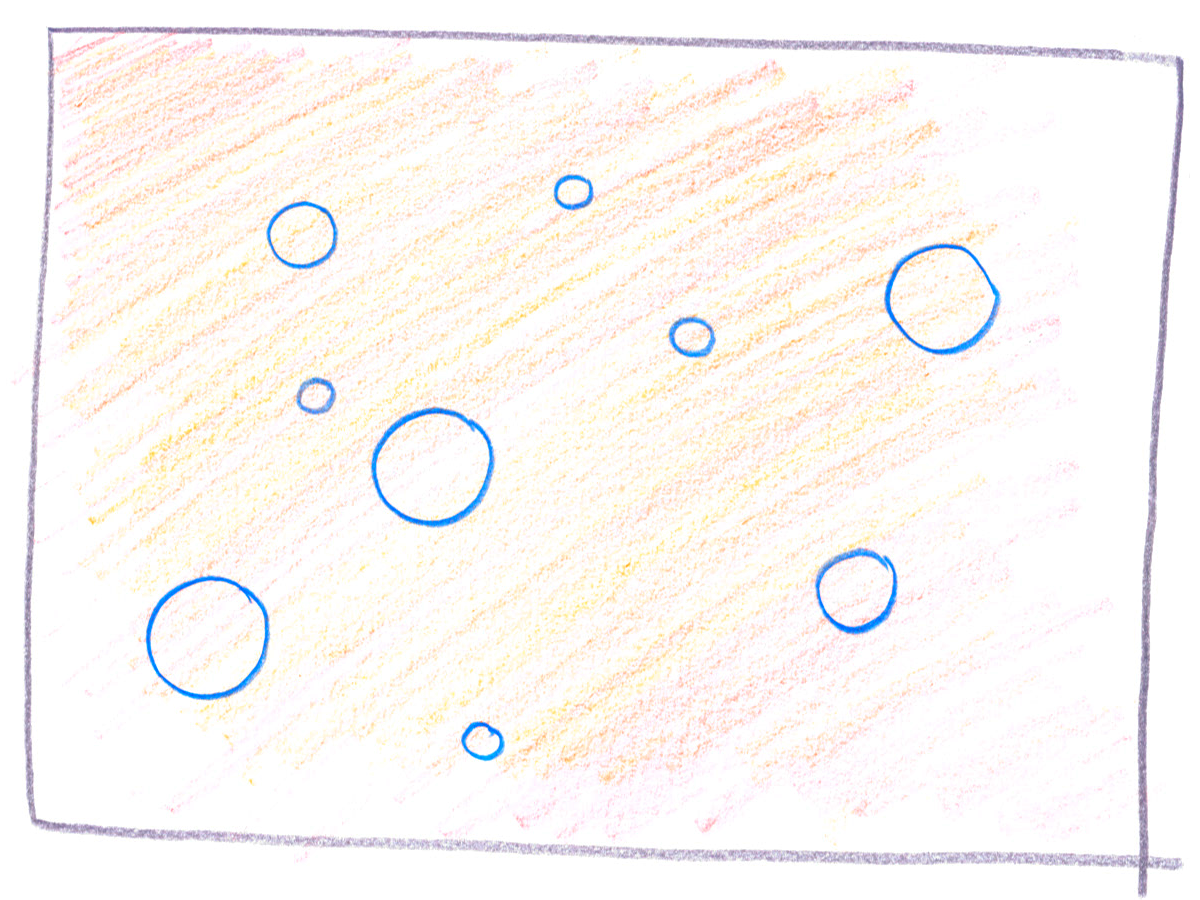
\includegraphics[width=\textwidth]{preliminary/visualizer_idea1.png}
\caption{A warm, light room with a high level of humidity}
\end{figure}

\begin{figure}
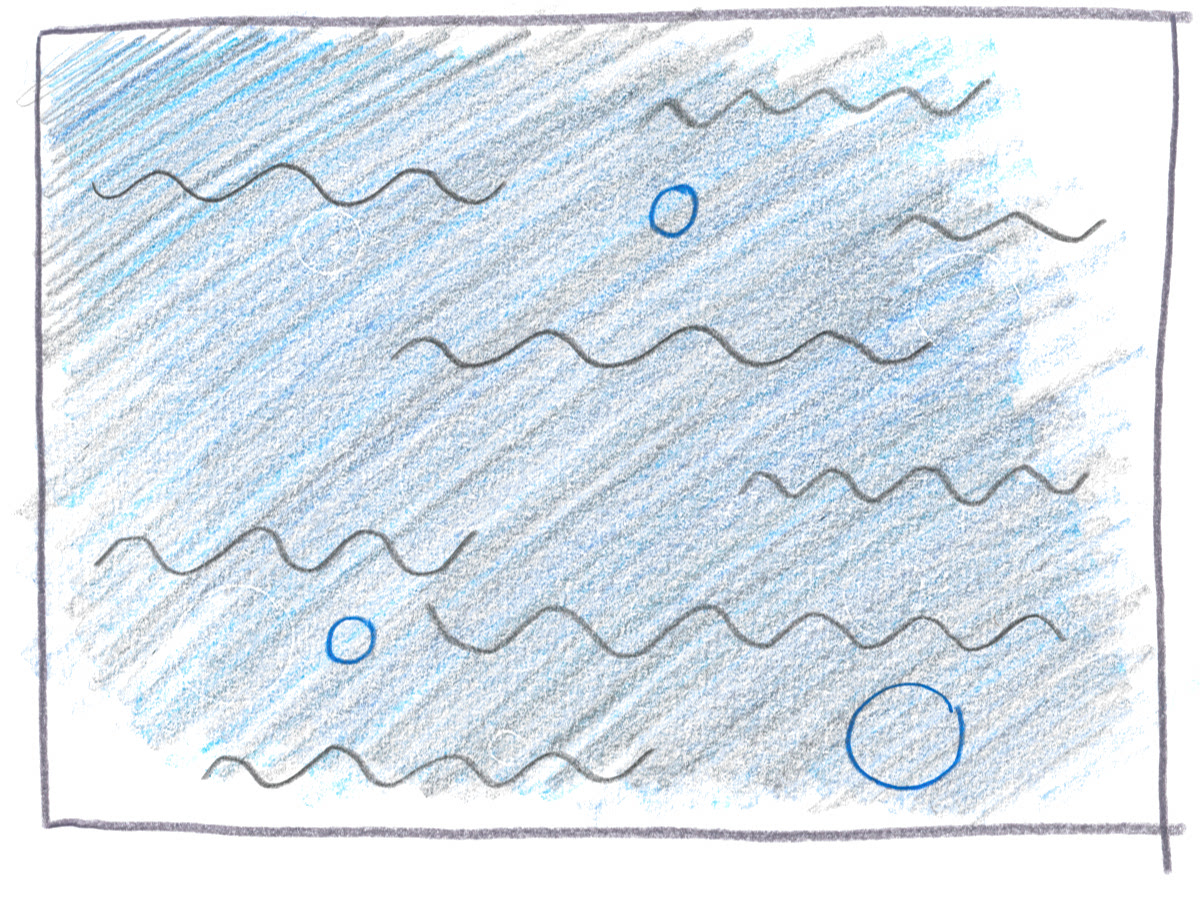
\includegraphics[width=\textwidth]{preliminary/visualizer_idea2.png}
\caption{A cold, dry and dark room with a high sound level}
\end{figure}

This idea is very simple to implement, however, it does not show data per sensor. It shows data as an average, which while it is good for some environments is unacceptable for others. Therefore this idea was quickly abandoned in favour of the next idea.

\subsection{Simple Image Manipulation in a grid}
Instead of having one image that would take all the data and average out the calculations, we would have a grid where a sensor or a group of sensors would provide the same image manipulation but on a grid scale.

While the grid solves the problems of whether individual sensors or a group of sensors are showing, it introduces another major problem. How to make the grid portable and modifiable. This was solved by using grid in a fairly “loose” meaning. Instead of it meaning a grid in its strict sense, the grid would be a sphere around each sensor. In this fashion the system can visualize a sensor’s immediate surrounding as well as average out values that overlap between two spheres. While this adds a layer of complexity to our implementation, we believe that it still remains fairly simple to implement.

\begin{figure}
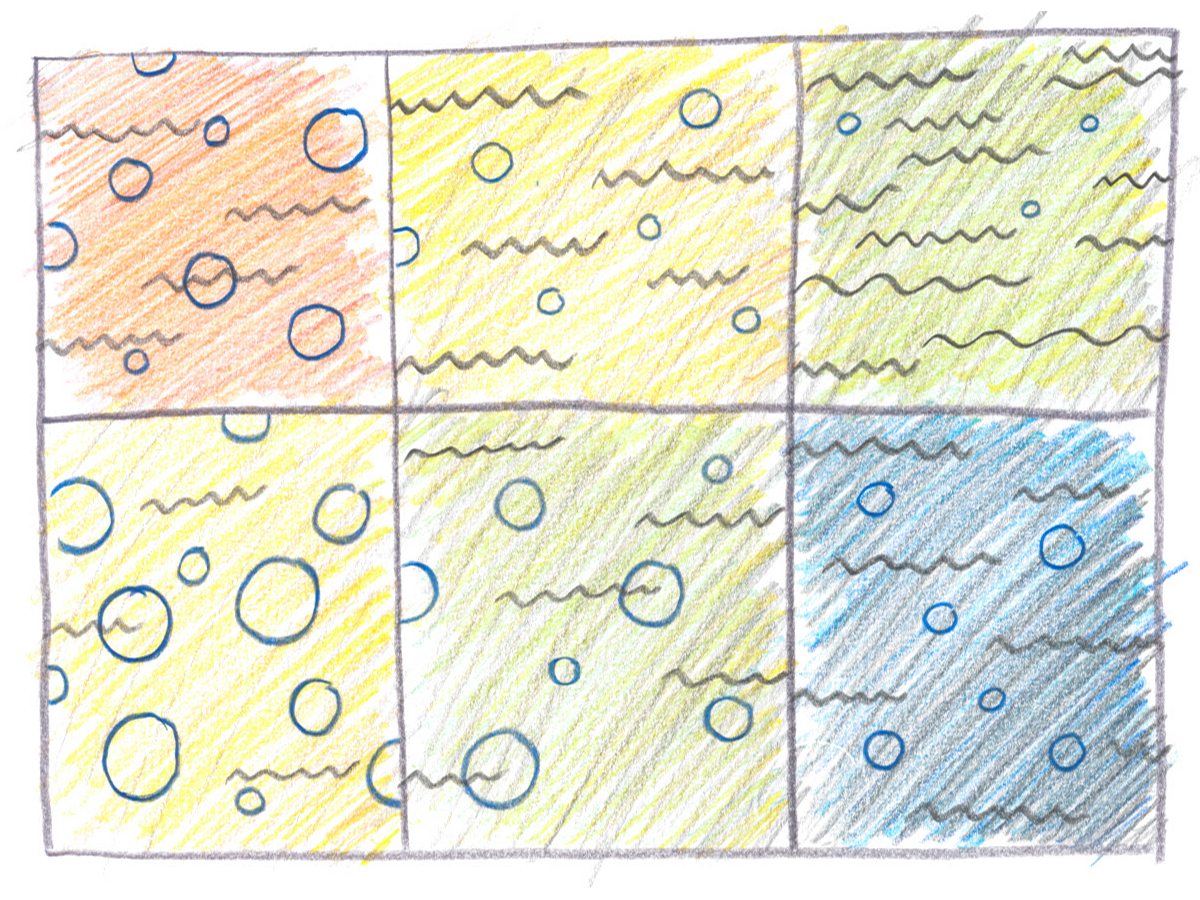
\includegraphics[width=\textwidth]{preliminary/visualizer_idea3.png}
\caption{Room visualisation with a grid}
\end{figure}

\begin{figure}
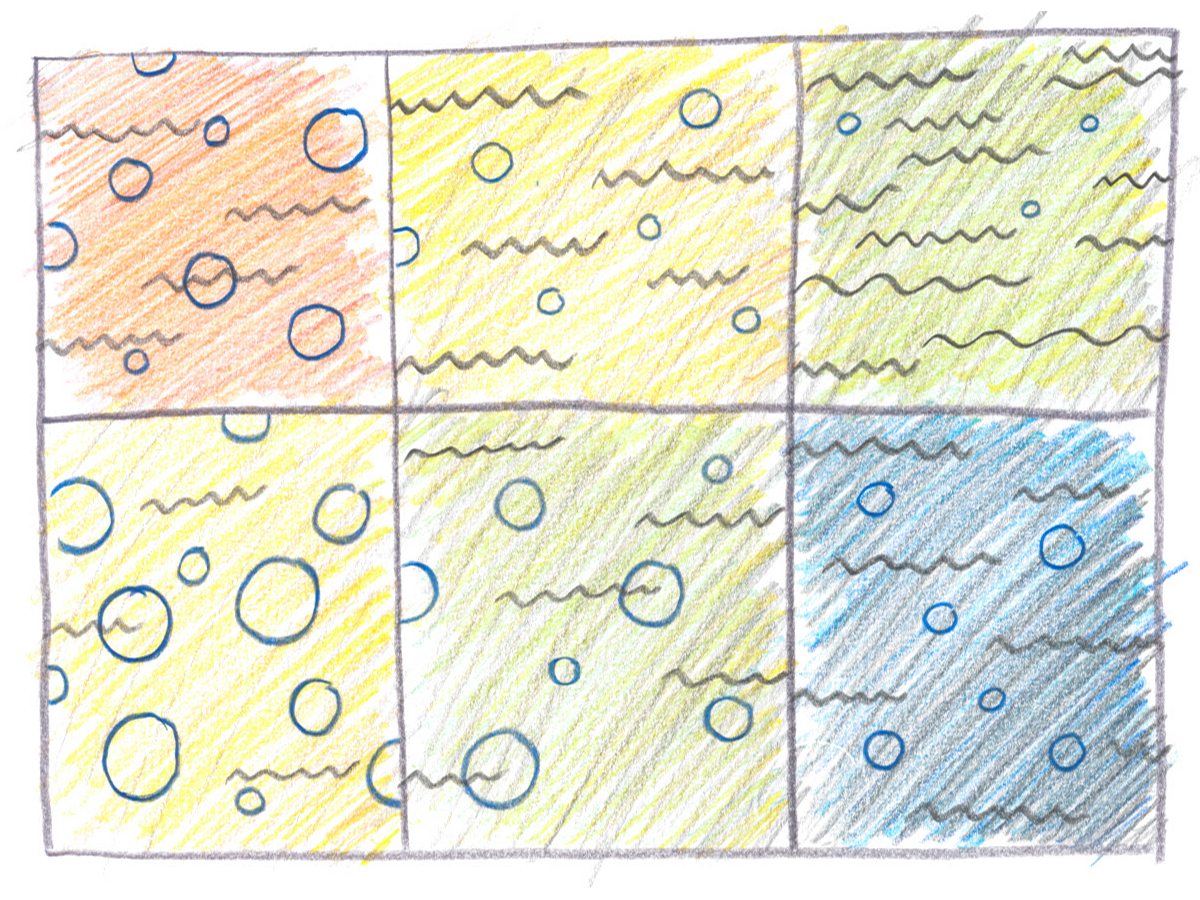
\includegraphics[width=\textwidth]{preliminary/visualizer_idea3.png}
\caption{Room visualisation with spheres}
\end{figure}

\subsection{Manipulation of sprites}
Instead of using geometrical shapes or simple colours, we can use small pre-made images commonly known as sprites. The system works in quite the same fashion. Every sensor or groups of sensors would be presented by a sprite, which would change based on the changes in the environment.

Sprites may be a bit more intuitive than colours and geometrical shapes, as they can speak more than the shapes can. For example a water sprite rising or lowering could represent the change in humidity. On the other hand it becomes more complex and time consuming to draw the sprites and even potentially animate them. Sprites also may have difficulty representing data that changes slowly, like temperature, and small changes to the data might be difficult to notice.

\begin{figure}
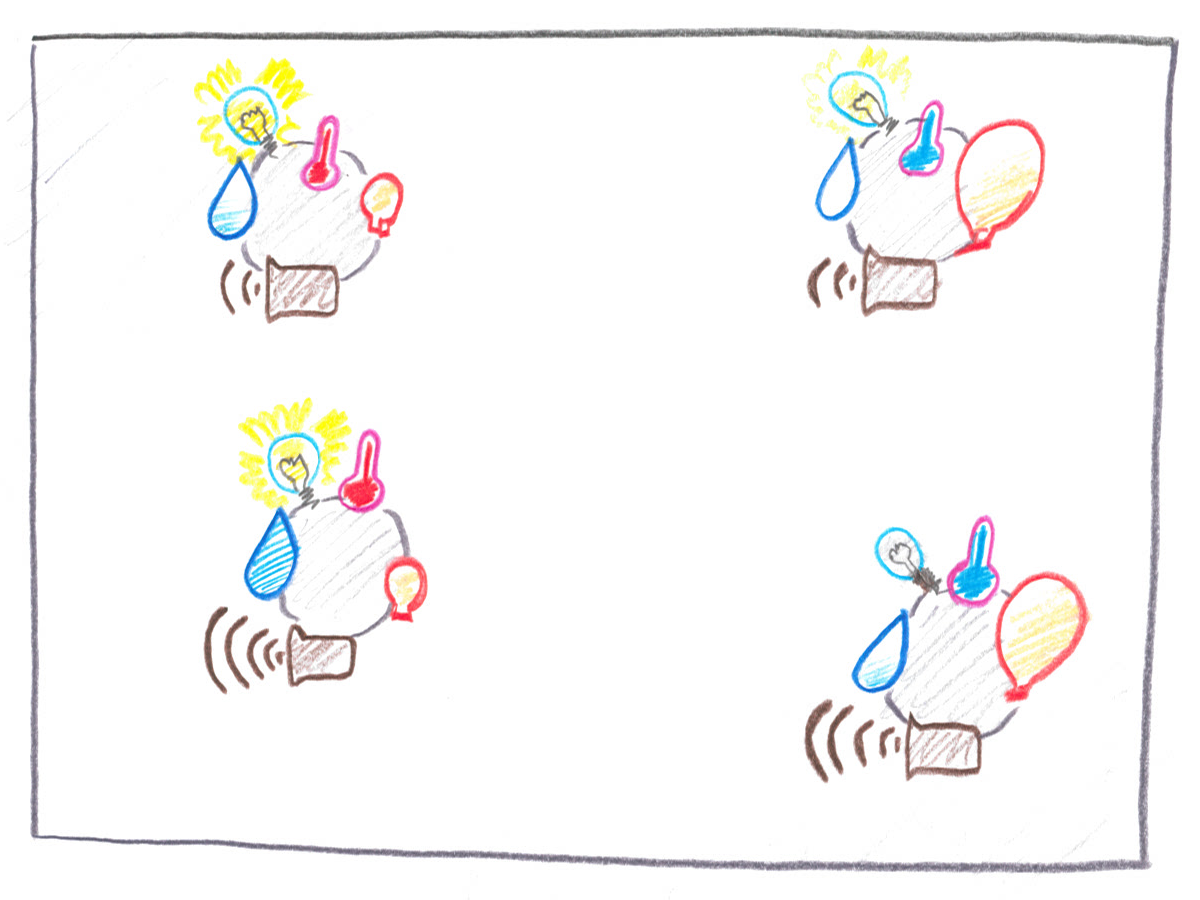
\includegraphics[width=\textwidth]{preliminary/visualizer_idea6.png}
\caption{Room visualisation with sprites}
\end{figure}

\begin{figure}
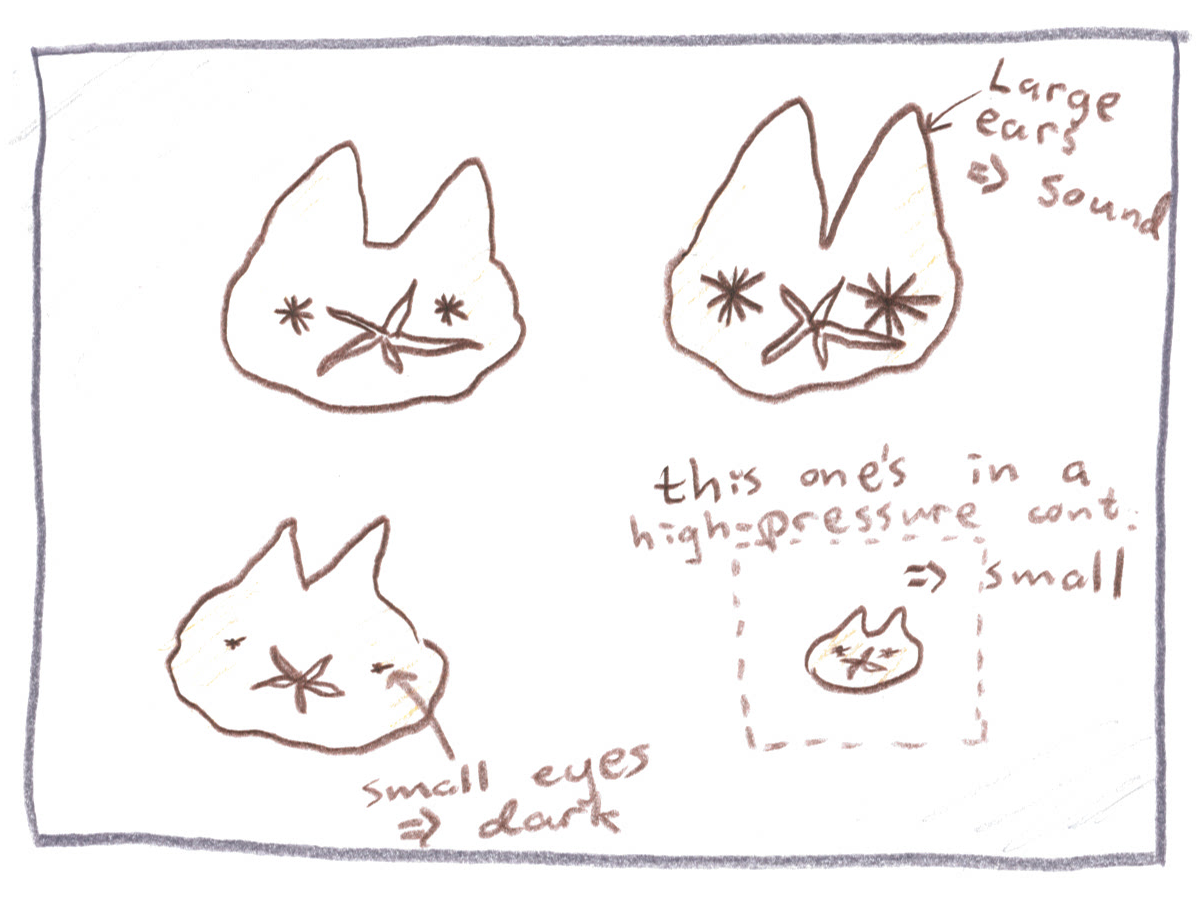
\includegraphics[width=\textwidth]{preliminary/visualizer_idea5.png}
\caption{Room visualisation with Potato Cat sprites}
\end{figure}

\end{document}